\problemname{Ég elska hana}

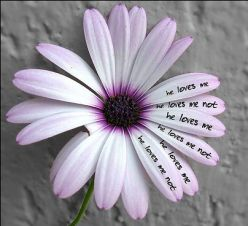
\includegraphics[width=0.4\textwidth]{flower.jpg}

\begin{quote}
Ég elska hana... ég elska hana ekki... ég elska hana...
\end{quote}

Jón litli var mjög hrifinn af Gunnu litlu. Hann horfði á hana sveifla sér í
rólunni úr fjarlægð, en hann var ekki ennþá búinn að þora að tala við hana.
Hann tekur upp blóm af jörðinni og byrjar að rífa af því laufblöðin. Hann tekur
fyrsta laufblaðið af blóminu og segir `Ég elska hana`. Svo tekur hann annað
laufblaðið af blóminu og segir þá `Ég elska hana ekki`. Jón skiptist á að
segja þessar tvær setningar þegar hann heldur áfram að rífa blöð af blóminu, og
gerir þetta þangað til hann heldur á síðasta laufblaðinu. Ef hann segir `Ég
elska hana` þegar hann heldur á síðasta laufblaðinu, þá ætlar hann loksins að
fara til Gunnu og segja henni hvað hann er hrifinn af henni. Annars ætlar hann
að halda áfram leika sér með hinum strákunum, og reyna aftur á morgun.

Inntakið inniheldur eina línu með heiltölunni $0 < n$ sem táknar fjölda
laufblaða á blóminu sem Jón litli tók upp af jörðinni. Úttakið á að innihalda
eina línu með setningunni sem Jón sagði þegar hann hélt á síðasta laufblaðinu,
sem er annaðhvort \texttt{Ég elska hana} eða \texttt{Ég elska hana ekki}.
